\PassOptionsToPackage{unicode}{hyperref}
\PassOptionsToPackage{naturalnames}{hyperref}
%\documentclass{beamer}
\documentclass[aspectratio=169, 12pt]{beamer}
\usepackage{hyperref}
\usepackage{color}
\usepackage{graphicx}
\usepackage{amsmath}
\usepackage{multirow}
\usepackage{array}
\usepackage{geometry}
\usepackage[utf8]{inputenc}
\usepackage{amssymb}
\usepackage{pifont}
\usepackage{marvosym}
\usepackage{makecell}
\usepackage{float}
\usepackage{multimedia}
\usepackage{listings}
\usepackage{MnSymbol,wasysym}
\usepackage{tikzpeople}
%\usepackage{setspace}
%\usepackage{utopia} %font utopia imported
\usefonttheme{professionalfonts}
%\usetheme{AnnArbor}
\usetheme{Berkeley}

\usecolortheme{default}

%------------------------------------------------------------
%This block of code defines the information to appear in the
%Title page
\title[Montgomery Hackathon 2021, Keynotes] %optional
{STEM, EECS \& A Little Touch on Cloud}

\subtitle{Montgomery Hackathon 2021 Keynotes}

\author[Changxu Luo] % (optional)
{
\texorpdfstring{\\Speaker: Changxu Luo, Software Engineer @Google}{}
\and
\texorpdfstring{\\\medskip\href{https://github.com/camelboat}{github.com/camelboat}}{}
}

\date[Summer 2021] % (optional)

%\logo{\includegraphics[height=0.3cm]{logo.jpg}}

%End of title page configuration block
%------------------------------------------------------------



%------------------------------------------------------------
%The next block of commands puts the table of contents at the 
%beginning of each section and highlights the current section:
%
%\AtBeginSection[]
%{
%  \begin{frame}
%    \frametitle{Table of Contents}
%    \tableofcontents[currentsection]
%  \end{frame}
%}
%%------------------------------------------------------------


\begin{document}

\definecolor{mGreen}{rgb}{0,0.6,0}
\definecolor{mGray}{rgb}{0.5,0.5,0.5}
\definecolor{mPurple}{rgb}{0.58,0,0.82}
\definecolor{backgroundColour}{rgb}{0.95,0.95,0.92}
\lstset{
    commentstyle=\color{mGreen},
    keywordstyle=\color{magenta},
    numberstyle=\tiny\color{mGray},
    stringstyle=\color{mPurple}\tt,
    basicstyle=\footnotesize,
    upquote=true,
    breakatwhitespace=false,
    breaklines=true,                 
    captionpos=b,         
    keepspaces=true,                 
    numbers=left,                    
    numbersep=5pt,                  
    showspaces=false,                
    showstringspaces=false,
    showtabs=true,                  
    tabsize=4,
    frame=tb,
    language=python,
    % basicstyle=\small\monaco]
}

%The next statement creates the title page.
\frame{\titlepage}
%---------------------------------------------------------
%This block of code is for the table of contents after
%the title page

\begin{frame}[fragile]
\frametitle{Outlines}
    \begin{columns}
        \column{0.3\textwidth}
            \tableofcontents
        \column{0.7\textwidth}
            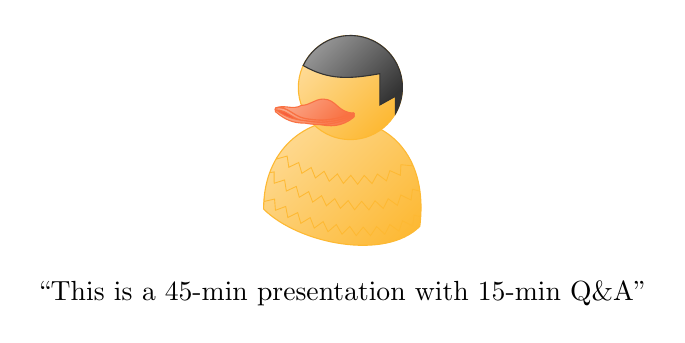
\begin{tikzpicture}[>=stealth]
            \node[duck, mirrored, minimum size=2cm, label=below:{``This is a 45-min presentation with 15-min Q\&A''}] (duck) at (0,0) {};
            \end{tikzpicture}
    \end{columns}
\end{frame}
%---------------------------------------------------------
\footnotesize
\section{A Little About Me}
\begin{frame}{A Little About Me}
\begin{itemize}
    \item BS in Electrical and Computer Engineering @Shanghai Jiaotong University
    \item MS in Electrical Engineering @Columbia University
    \item Worked as Software/Electrical Engineer @GE Appliances, Bosch, and Rover Diagnostics
    \medskip
    \item Software Engineer @Google - Google Cloud Networking Control Qualification
    \item Research Assistant on distributed storage, instructed by Prof. Asaf Cidon.
\end{itemize}
\end{frame}

\begin{frame}{A Little About Me, Cont.}
    \begin{figure}
        \centering
        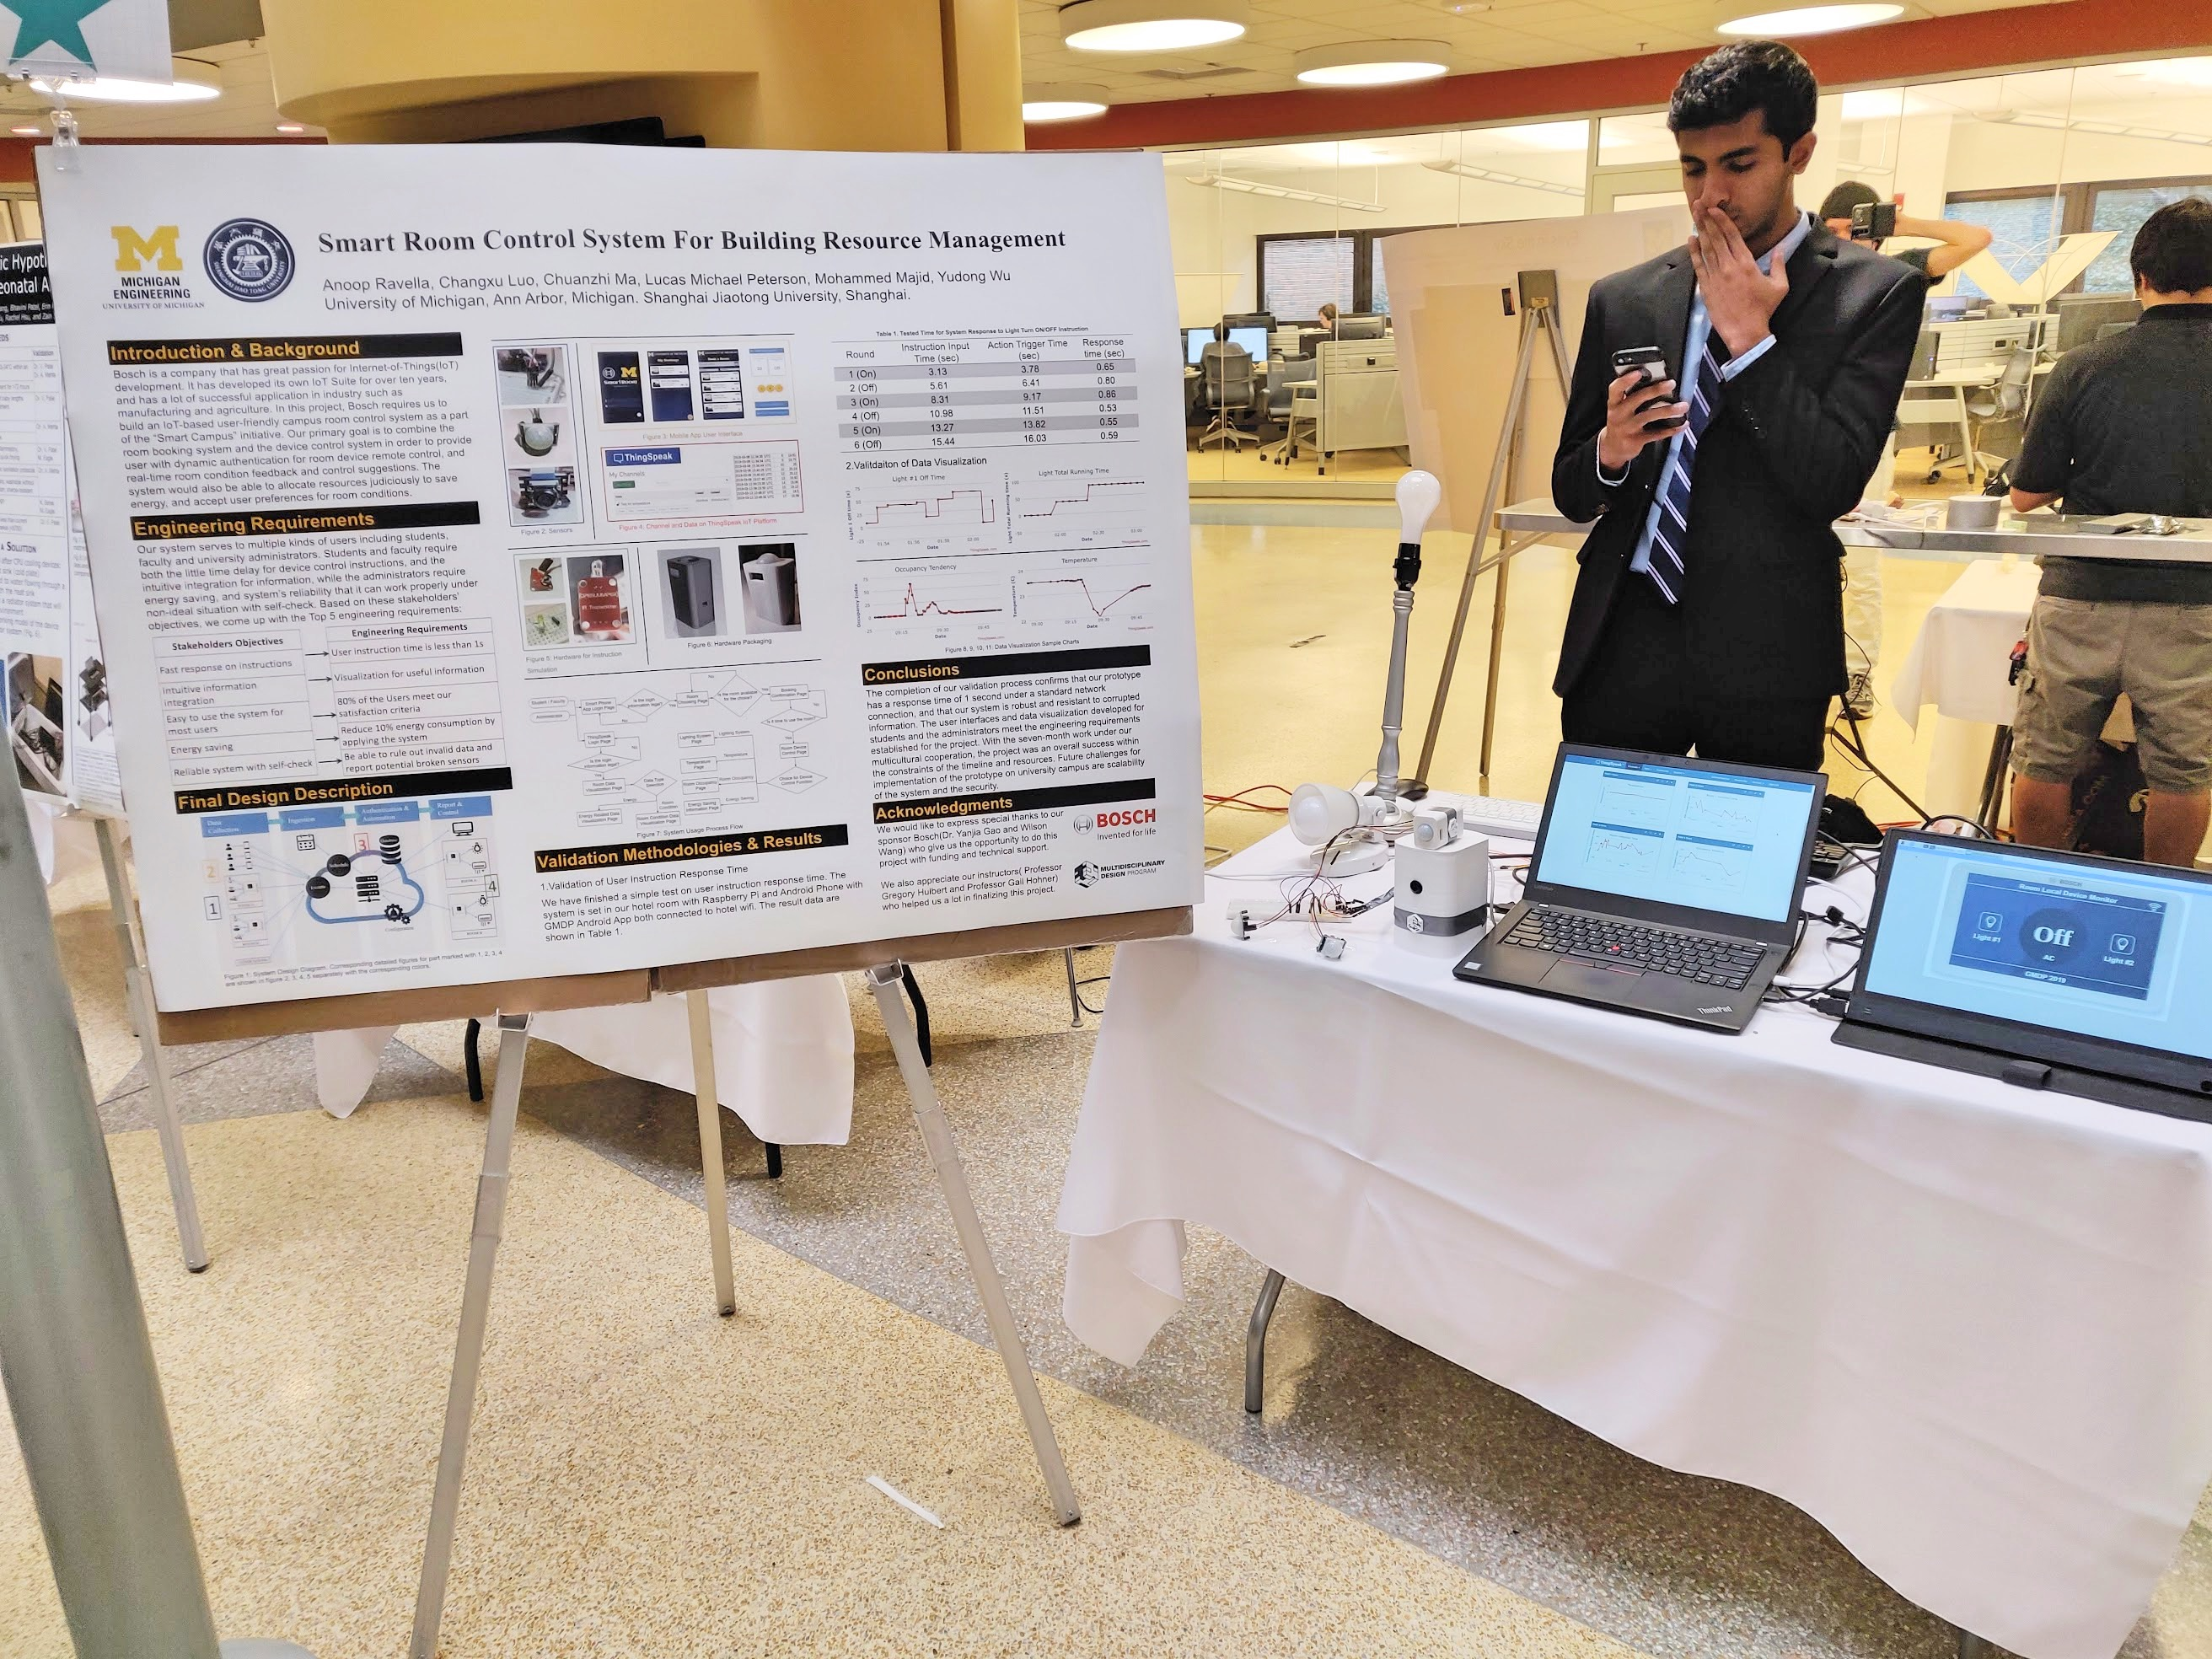
\includegraphics[width=0.6\textwidth]{assets/GMDP.jpg}
        \caption{Project Expo at UMich}
        \label{fig:GMDP}
    \end{figure}
\end{frame}

\begin{frame}{A Little About Me, Cont.}
    \begin{figure}
        \centering
        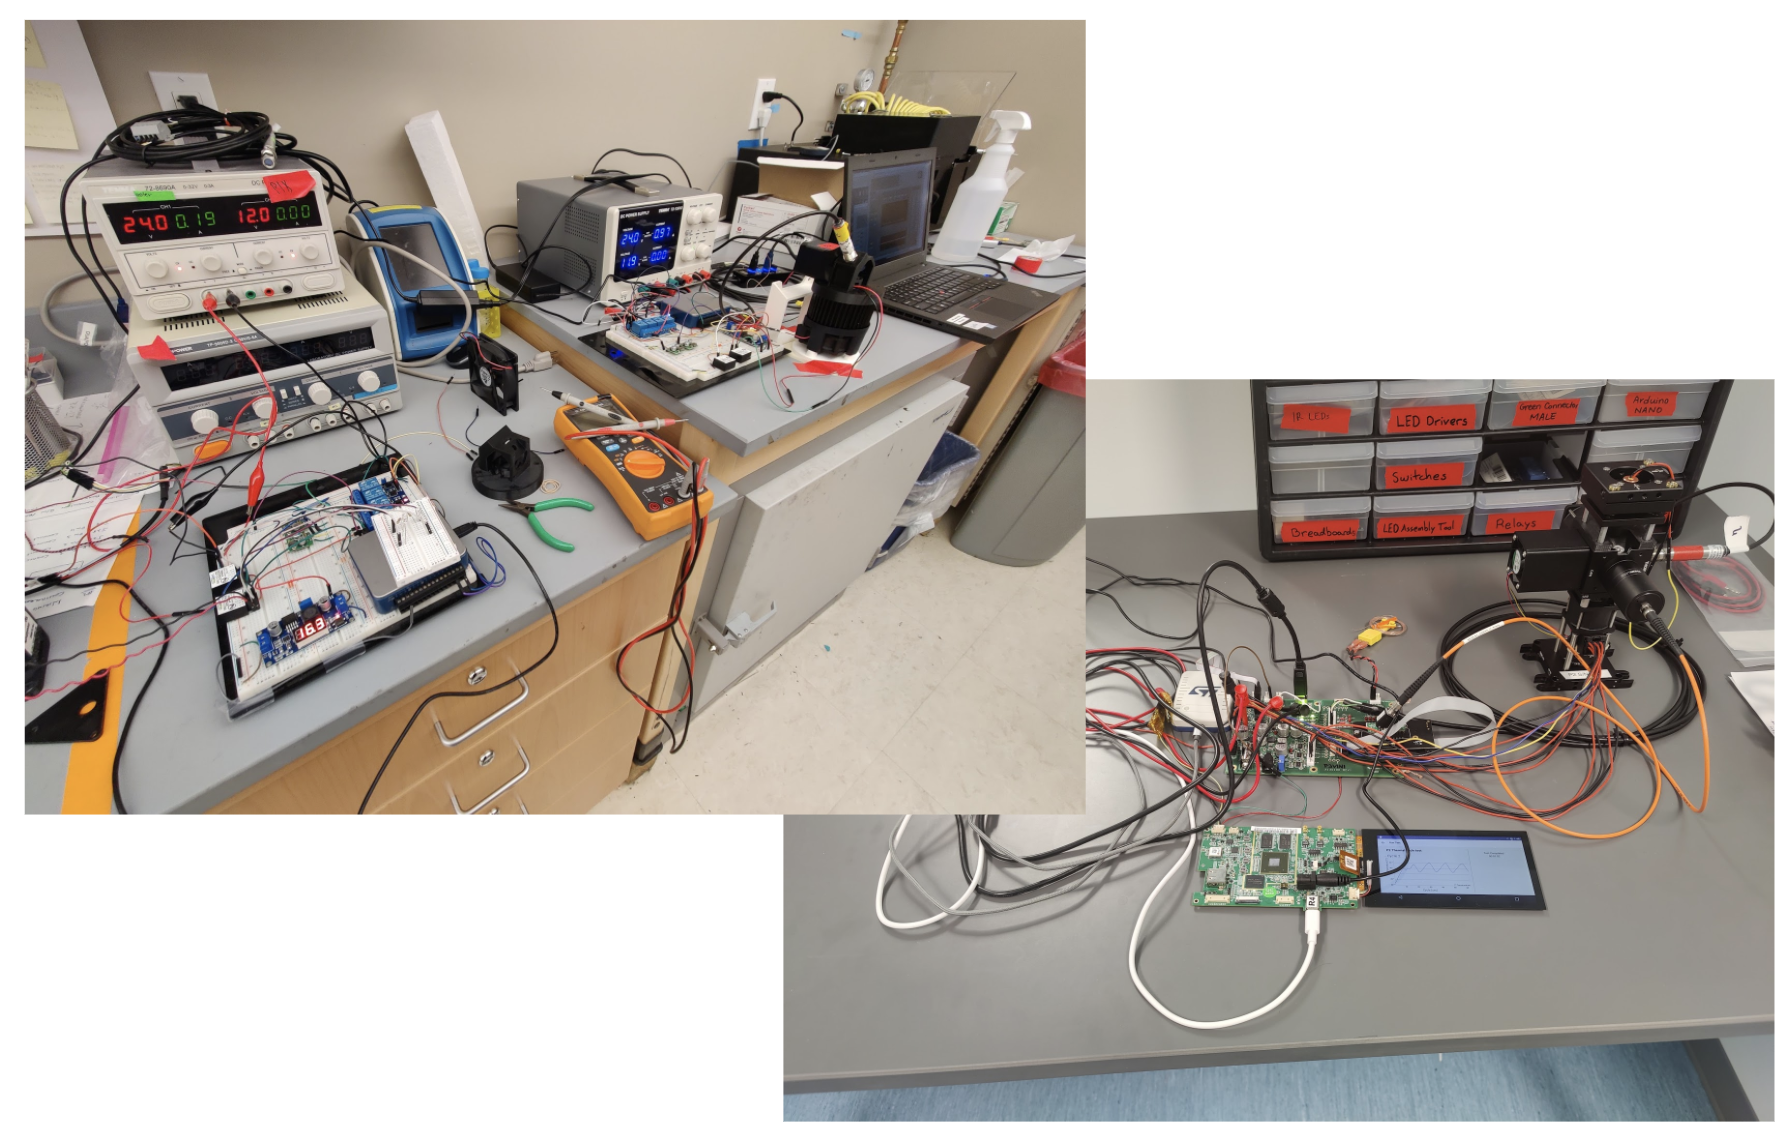
\includegraphics[width=0.7\textwidth]{assets/Rover_3.png}
        \caption{Prototypes developed at Rover Diagnostics}
        \label{fig:Rover}
    \end{figure}
\end{frame}

\begin{frame}{A Little About Me, Cont.}
    At Google, I've worked for two teams:
    \begin{enumerate}
    \item Assistant and Search(internship, Google Assistant Feature Development for Google Home)
    \item Google Cloud Platform(current position, GCP Networking Release Qualification Framework)
    \end{enumerate}
    \medskip
    No worries, you don't have to understand my work now \smiley{} 
    \\\medskip(and I am not able to show you any details \frownie{}, but wait for the second session for the Cloud ice-breaker!)
\end{frame}


\section{STEM/EE/CS?}
\begin{frame}{STEM?}

\begin{tikzpicture}[>=stealth]
\node[alice, minimum size=2cm,label=below:{``What is STEM?''}] (alice) at (0,0) {};
%\node[bob, mirrored, minimum size=2cm, right=5cm of alice, label=below:{''Good questions, let's see the definition''}] (bob) {};
%\node[bob, mirrored, minimum size=2cm, right=5cm of alice, label=below:{Bob: $K, b$}] (bob) {};
%\draw[->,thick] (alice.20) -- node[above]{$E(g^a\ \text{mod}\ p, K)$} (bob.160);
%\draw[<-,thick] (alice.-20) -- node[above]{$E(g^b\ \text{mod}\ p, K)$} (bob.-160);
\end{tikzpicture}
\end{frame}

\begin{frame}{STEM?}

\begin{tikzpicture}[>=stealth]
\node[alice, minimum size=2cm,label=below:{``What is STEM?''}] (alice) at (0,0) {};
\node[duck, mirrored, minimum size=2cm, right=8cm of alice, label=below:{``I am glad you asked!''}] (duck) {};
%\node[bob, mirrored, minimum size=2cm, right=5cm of alice, label=below:{Bob: $K, b$}] (bob) {};
%\draw[->,thick] (alice.20) -- node[above]{$E(g^a\ \text{mod}\ p, K)$} (bob.160);
%\draw[<-,thick] (alice.-20) -- node[above]{$E(g^b\ \text{mod}\ p, K)$} (bob.-160);
\end{tikzpicture}
\end{frame}

\begin{frame}{STEM? Cont.}
\begin{block}{STEM}
Science, technology, engineering, and mathematics(STEM), a term to group together these academic disciplines\footnote{\tiny\url{https://fas.org/sgp/crs/misc/R42642.pdf}}.
\end{block}

\begin{block}{ And if we name some of those disciplines(with the narrow definition\footnote{\tiny In a general definition, all these disciplines can be a form of science, such as Formal Science(Math), Natural science(Physics, Chemistry), Applied science(Engineering)})}
\begin{itemize}
\item Science: Physics, Chemistry, \textbf{Computer Science}, etc.
\item Engineering: \textbf{Electrical Engineering}, Computer Engineering, Mechanical Engineering, etc.
\item Mathematics: Mathematics
\end{itemize}
\end{block}
\end{frame}

\begin{frame}{STEM? EE? CS?}
\begin{alertblock}{Relations of Science, Technology, Engineering, and Math(with the narrow definition)}
\begin{enumerate}
\item Math is the language for describing science(study of the natural world).
\item Engineering is the systematic and iterative approach to the human applications of science.
\item Technologies are those applications.
\end{enumerate}
\end{alertblock}
\end{frame}

\begin{frame}{STEM? Cont.}
\centering
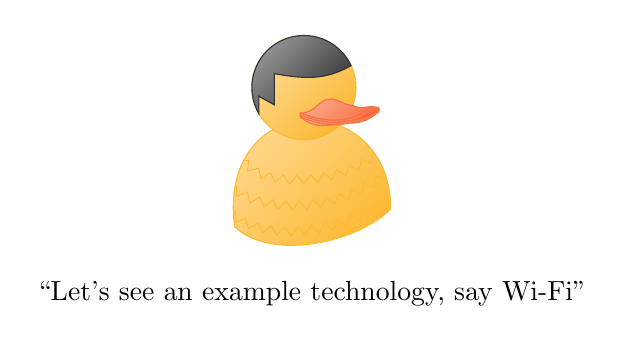
\begin{tikzpicture}[>=stealth]
\node[duck, minimum size=2cm, label=below:{``Let's see an example technology, say Wi-Fi''}] (duck) at (0,0) {};
\end{tikzpicture}
\end{frame}

\begin{frame}{STEM? Cont.}
    \begin{columns}
        \column{0.3\textwidth}
            \centering
            
\begin{tikzpicture}[>=stealth]
            \node[duck, minimum size=2cm, label=below:{``What's Wi-Fi?''}] (duck) at (0,0) {};
            \end{tikzpicture}
        \column{0.7\textwidth}
            \begin{block}{Wi-Fi}
            \begin{itemize}
            \item A family of wireless network protocols, based on the IEEE 802.11 family of standards.
            \item Allowing nearby digital devices to exchange data by radio waves.
            \end{itemize}

            \end{block}
    \end{columns}
\end{frame}

\begin{frame}{A VERY brief overview for Wi-Fi knowledge stack}
    \begin{figure}
        \centering
        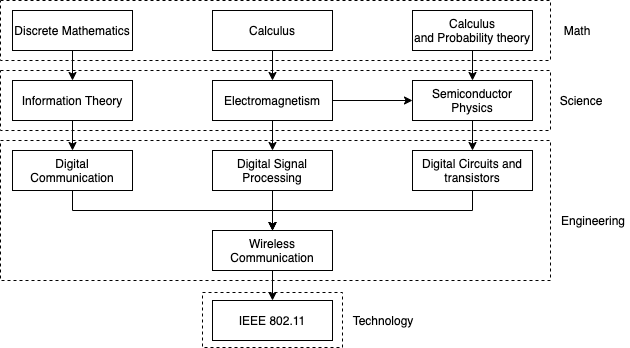
\includegraphics[width=0.8\textwidth]{assets/wifi.png}
        \label{fig:wifi}
    \end{figure}
\end{frame}

\begin{frame}{A VERY brief overview for Wi-Fi knowledge stack, Cont.}
    \begin{figure}
        \centering
        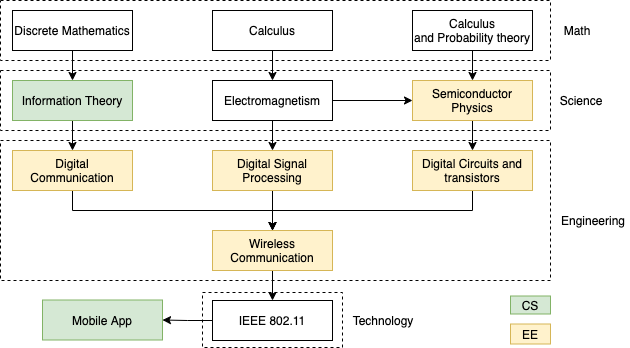
\includegraphics[width=0.8\textwidth]{assets/wifi_2.png}
        \label{fig:wifi2}
    \end{figure}
\end{frame}

\begin{frame}{EE, Overview by Phrases\footnote{\tiny If you want to have a more details among which courses should you expect to take in EECS, visit the curriculum map at \url{https://ocw.mit.edu/courses/mit-curriculum-guide/}}}
\begin{block}{Electrical Engineering}
Study, design and application of equipment, devices and systems which use electricity, electronics, and electromagnetism.
\end{block}
\begin{itemize}
\scriptsize
\item Computer Engineering(often an individual discipline nowadays)
\item Automation and Control
\item Power and Energy
\item Electronics
\item Telecommunications
\item Signal Processing
\item Optics and Photonics
\footnote{\tiny I simply copy them from Wikipedia, not a strict catalog.}
\end{itemize}
\end{frame}

\begin{frame}{CS, Overview by Phrases}
\begin{block}{Computer Science}
Study of algorithmic processes, computational machines and computation itself\footnote{\tiny\url{https://www.cs.york.ac.uk/undergraduate/what-is-cs/}}.
\end{block}
\begin{itemize}
\scriptsize
\item Theoretical computer science(Computation Theory, Information and coding theory, Data structures and algorithms, Programming language theory and formal methods, etc.)
\item Computer systems and computational processes(Artificial Intelligence, Computer architecture and organization, Concurrent, parallel and distributed computing, Computer networks, Cryptography, Databases, Graphics, etc.)
\item Applied computer science(computational science, finance and engineering, software engineering, social computing and human-computer interaction, etc.)
\end{itemize}
\end{frame}

\begin{frame}{The Magic of EECS}
    \begin{columns}
        \column{0.3\textwidth}
            \centering
            
\begin{tikzpicture}[>=stealth]
            \node[duck, good, minimum size=2cm, label=below:{``Magic!''}] (duck) at (0,0) {};
            \end{tikzpicture}
        \column{0.7\textwidth}
            To me(as well as many others), the magic of EECS is that for the first time in human history, it frees us from following the restriction of physical laws and allows us to create and present the logics that is never seen before(just think about any video games!), and applies the logics that can be proved before(for math development).
            \\\medskip
            And as a student in EECS, you can be part of the magic!
    \end{columns}
\end{frame}

\begin{frame}{The Magic of EECS\footnote{\tiny I found a great video made by Intel for the introduction of making a microchip: \url{https://www.youtube.com/watch?v=_VMYPLXnd7E}}}
    \begin{figure}
        \centering
        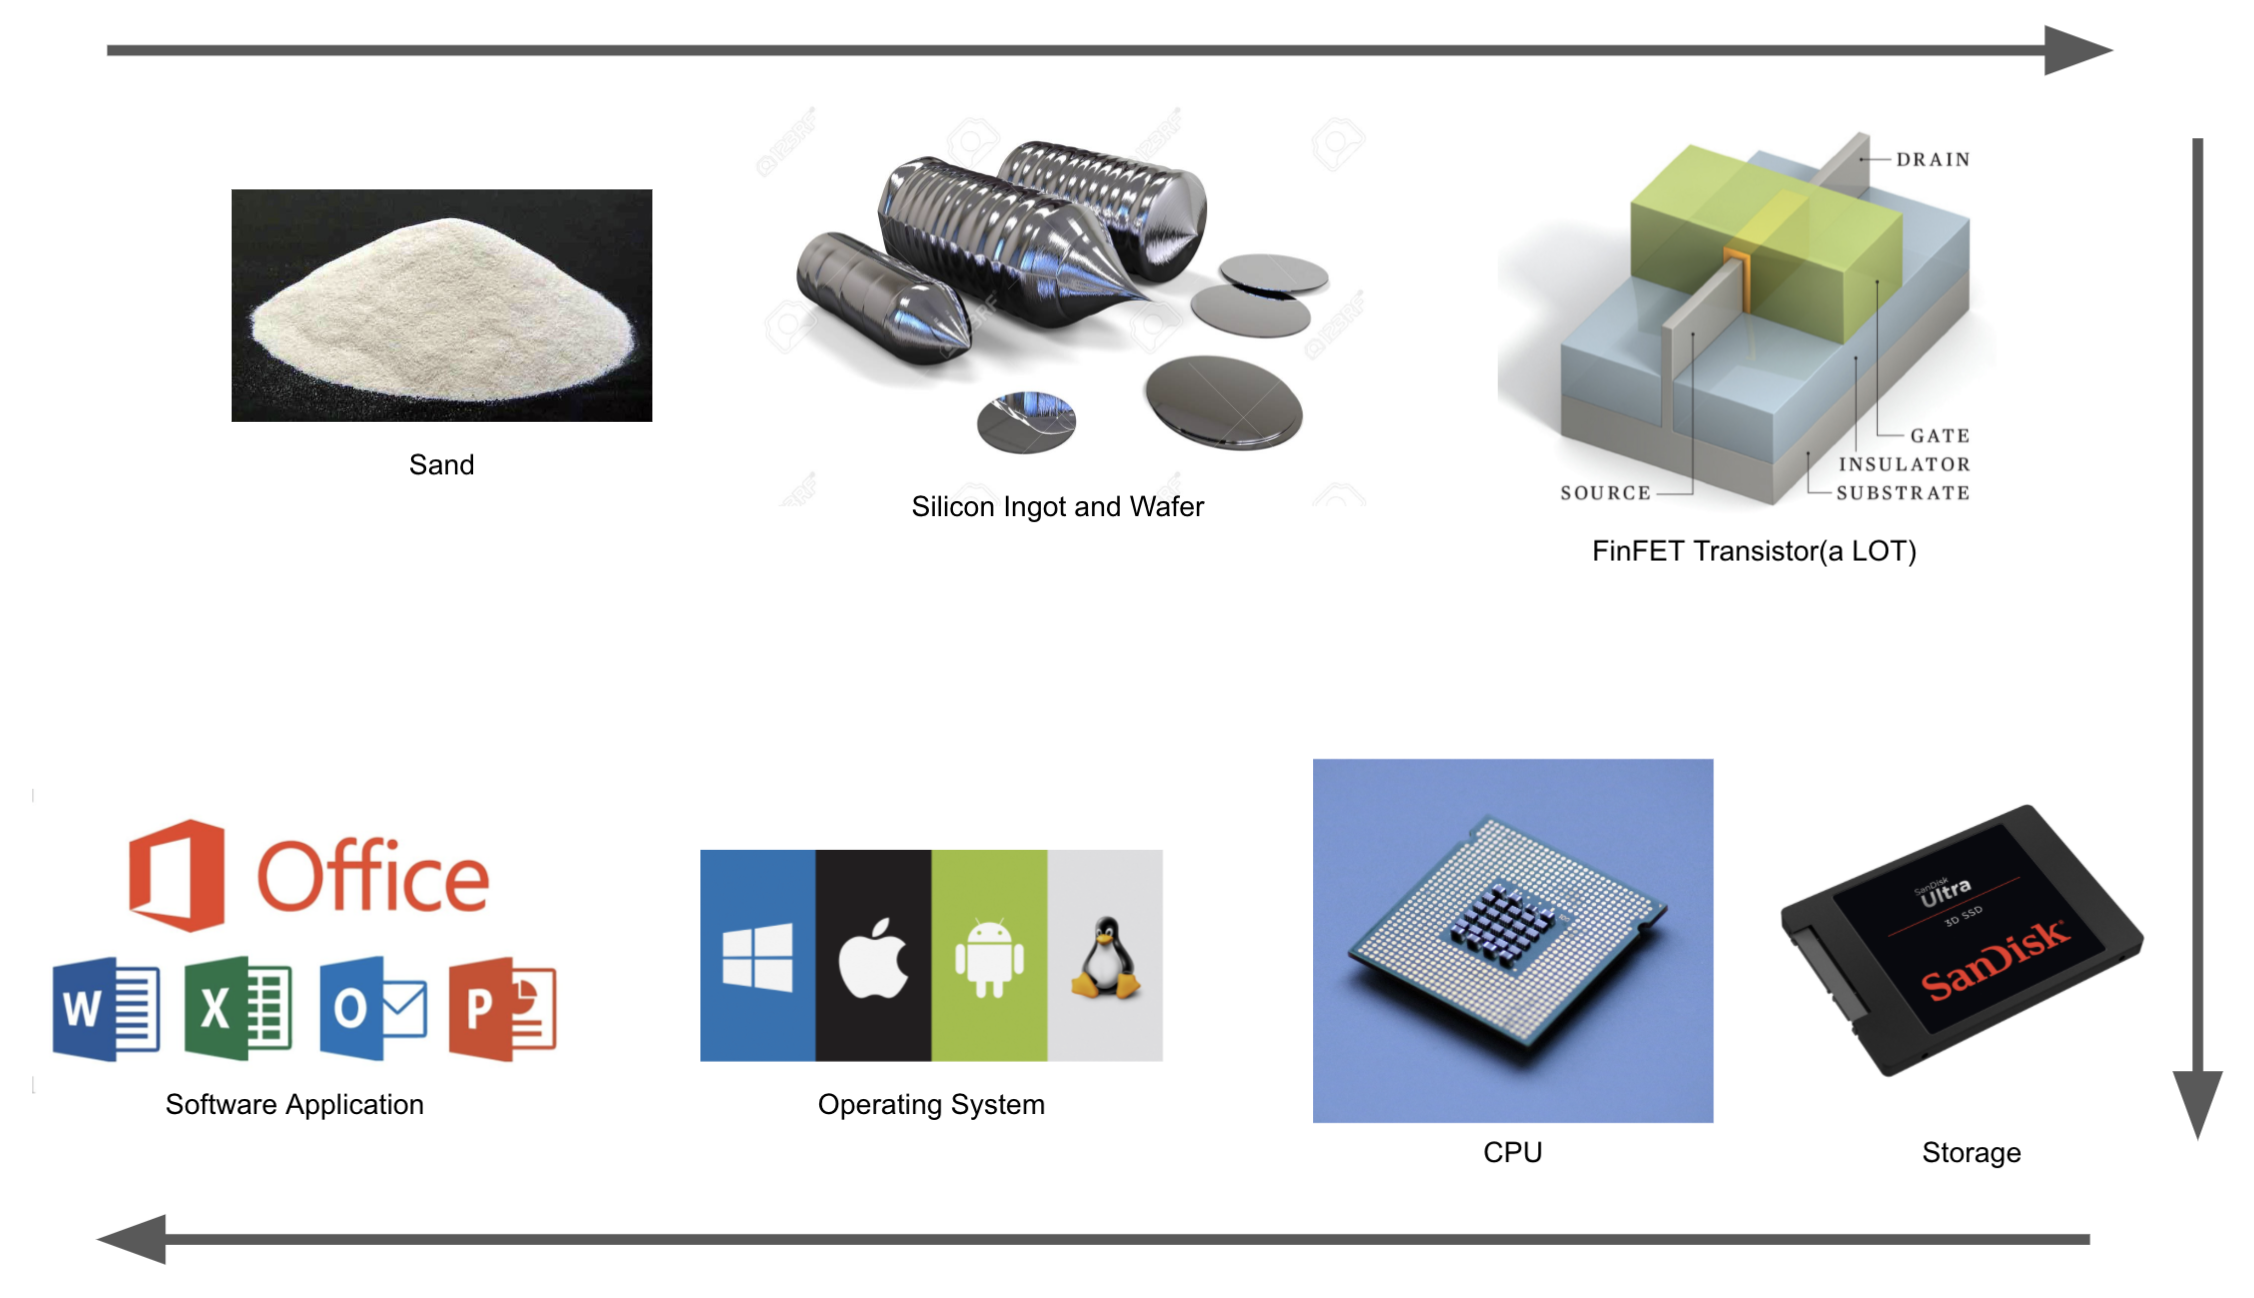
\includegraphics[width=0.8\textwidth]{assets/magic.png}
        \label{fig:magic}
    \end{figure}
\end{frame}

\begin{frame}[fragile]{Why EE? Why CS?}
In EE, you can learn how to manipulate the electrics physical laws and how it grows until something that can bear pure logics(Sand$\rightarrow$Instruction Code, Signal$\rightarrow$Digital Data).
$$\downarrow$$
\begin{lstlisting}[upquote=true]
def main():
  print('Hello world!')

if __name__ == '__main__':
  main()
\end{lstlisting}
$$\downarrow$$
In CS, you can then learn to extend this logic and make system that is large-scale, complex, based on the human logic laws(system interfaces) instead of physical laws.
\end{frame}

\begin{frame}{Why EE? Why CS?}
Of course, this is not the whole story, since EE and CS are considered together in so many ways. Just name two:
\begin{itemize}
\item The signal processing requires complex algorithms and computer science theories, and before applying all the fancy artificial intelligence algorithms, it is better for you to understand what is happening in the physical world.
\item Programmer needs sophisticated understanding on hardware in order to get the best software performance. For beginners, you may feel like the resources on a system is unlimited, unfortunately, they are limited\footnote{\tiny This is a hard job which is pursued by a lot of advanced software community like operating system, scientific computing, and programming languages communities.}.
\end{itemize}
\end{frame}

\begin{frame}{Why EE? Why CS?}
    \begin{columns}
        \column{0.3\textwidth}
            \centering
            
\begin{tikzpicture}[>=stealth]
            \node[duck, minimum size=2cm, label=below:{``This is a good time!''}] (duck) at (0,0) {};
            \end{tikzpicture}
        \column{0.7\textwidth}
            Thanks to the development of computation hardware and open-source communities, we have prototyping hardwares and software tools that are highly accessible.
    \end{columns}
\end{frame}



\begin{frame}{Resources to Get Started!}
\begin{block}{Prototype Hardware}
\begin{itemize}
\item Arduino
\item Raspberry Pi
\end{itemize}
\end{block}

\begin{block}{Workstation}
\begin{itemize}
\item Any personal device with a browser\footnote{\tiny Maybe also a USB port.}!(thanks to the cloud services)
\end{itemize}

\end{block}
\begin{block}{What Language to Learn}
\begin{itemize}
\item TL;DR, Python, or follow your course instructors
\end{itemize}
\end{block}
\end{frame}

\begin{frame}{Recourses to Get Started! Cont.}
\begin{block}{Documents}
\begin{itemize}
\item Go to your target's official website and follow the tutorial.
\item Search engine is powerful.
\end{itemize}
\end{block}

\begin{block}{Sites you want to know as a beginner}
\begin{itemize}
\item \url{github.com}
\item \url{colab.research.google.com}, run Python notebook on cloud freely
\item \url{codepen.io}, front-end dev playground
\end{itemize}
\end{block}
\end{frame}

\begin{frame}{Recourses to Get Started! Cont.}
\centering

\begin{tikzpicture}[>=stealth]
\node[duck, evil, monitor, minimum size=2cm, label=below:{``And feel free to reach out me!''}] (duck) at (0,0) {};
\end{tikzpicture}
\centering
\\\medskip
\href{mailto:changxu.luo@columbia.edu}{changxu.luo@columbia.edu}
\end{frame}

%\begin{frame}{Electrical Engineering?}
%    \centering
%    \movie[externalviewer]{\includegraphics[width=\textheight, keepaspectratio]{assets/Columbia_ss.png}}{/Users/camelboat/Desktop/Columbia.mov}
%\end{frame}

\section{What is Cloud?}
\begin{frame}{What is Cloud? Taking Cloud Gaming as an Example}
\centering
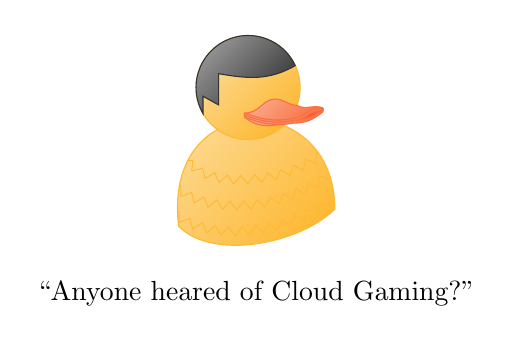
\begin{tikzpicture}[>=stealth]
\node[duck, minimum size=2cm, label=below:{``Anyone heared of Cloud Gaming?''}] (duck) at (0,0) {};
\end{tikzpicture}
\end{frame}

\begin{frame}{What is Cloud? Cont.}
\centering
    \begin{figure}
        \centering
        
\includegraphics[width=0.8\textwidth]{assets/cloud_gaming.png}
        \label{fig:cloudgaming}
    \end{figure}
\end{frame}

\begin{frame}{What is Cloud? Taking Cloud Gaming as an Example Cont.}
As a normal consumer(gamer), what is different with the cloud gaming service?
\scriptsize
\begin{alertblock}{Without Cloud Gaming}
\begin{itemize}
\item You buy a PS5/gaming PC.
\item You buy and download Celesta.
\item You start playing Celesta and the game(computation) is running mainly on your local machine.
\end{itemize}
\end{alertblock}

\begin{alertblock}{With Cloud Gaming}
\begin{itemize}
\item You have a machine with Chrome.
\item You buy Stadia membership.
\item You start playing Celesta and the game(computation) is running mainly on Google's service with the video data streaming to your machine.
\end{itemize}
\end{alertblock}
\end{frame}

\begin{frame}{What is Cloud? Taking Cloud Gaming as an Example Cont.}
As a (normal)gamer, what is your main purpose?
\begin{itemize}
\item \ding{55} Maintain and upgrade your hardware.
\item \ding{55} Save, load, and maintain gaming data manually.
\item \ding{51} Play the game(have the accessory input and get visual/sound feedback).
\end{itemize}
\vfill
Cloud gaming maintain the most expensive hardware and backup data for you and let you focus on the game itself\footnote{\tiny Current cloud gaming services still have their problem like the requirement to the networking conditions, but they also have other benefits as a cloud services}.
\end{frame}

\begin{frame}{Cloud for Developer}
Now let's say you are a developer, what is your main purpose?
\begin{itemize}
\item \ding{55} Maintain and upgrade your hardware and infrastructure(server, networking, data center place, etc.)
\item \ding{55} Maintain your business data manually(backup, recover, anti-hacking)
\item \ding{51} Implement the business logic\footnote{\tiny Just think of business logic as the normal application logic, i.e., the code you write} for the application and get the things done.
\end{itemize}
\vfill
Cloud services maintain the infrastructure for you(with a lot of helpful services like load-balancing, authentication, data storage, deployment, etc.) and let the developer focus on their application's business logic.
\end{frame}

\begin{frame}{Cloud for Developer}
\centering
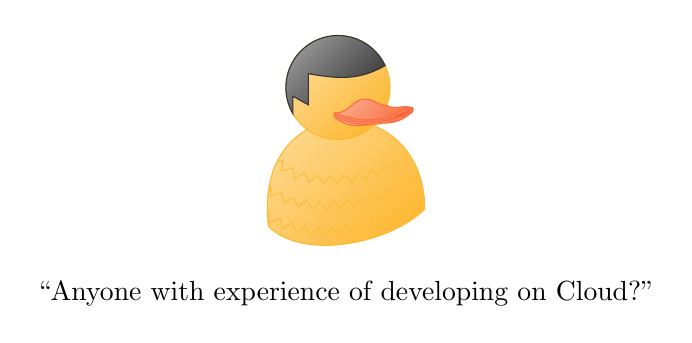
\begin{tikzpicture}[>=stealth]
\node[duck, minimum size=2cm, label=below:{``Anyone with experience of developing on Cloud?''}] (duck) at (0,0) {};
\end{tikzpicture}
\end{frame}

\begin{frame}{Cloud for Developer}
    \begin{figure}
        \centering
        
\includegraphics[width=0.8\textwidth]{assets/cloud.png}
        \label{fig:cloud}
    \end{figure}
\end{frame}

\begin{frame}{DEMO}
\Huge Launch a web app on AWS 
\\\medskip
in 5 mins!
\end{frame}

\begin{frame}{Rambling}
\centering
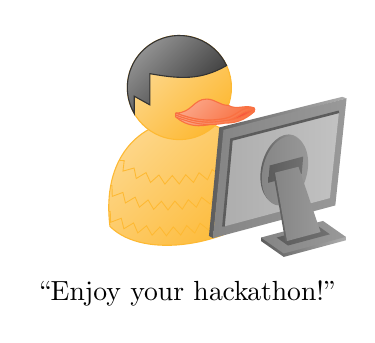
\begin{tikzpicture}[>=stealth]
\node[duck, monitor, minimum size=2cm, label=below:{``Enjoy your hackathon!''}, font=\Large] (duck) at (0,0) {};
\end{tikzpicture}
\vfill
\centering
\begin{itemize}
\scriptsize
\item Demo is fun and easy, research and production are hard, but try to keep your passion.
\item If you want to go STEM, or even go EECS, try to find what's your passion among hundreds of subfields. Go broad, and then go top.
\item Start your first project now!
\end{itemize}
\end{frame}

\begin{frame}{Q\&A}
\centering

\begin{tikzpicture}[>=stealth]
\node[duck, shield, sword, minimum size=2cm, label=below:{``Ask me anything''}] (duck) at (0,0) {};
\end{tikzpicture}
\vfill
\centering
\href{mailto:changxu.luo@columbia.edu}{changxu.luo@columbia.edu}
\\\medskip
\href{https://github.com/camelboat}{github.com/camelboat}
\\\medskip
\tiny Find this slide at \href{https://github.com/camelboat/Montgomery_Hackathon_2021_Keynote_Speech/blob/master/Slides.pdf}{github.com/camelboat/Montgomery\_Hackathon\_2021\_Keynote\_Speech/blob/master/Slides.pdf}
\end{frame}

\begin{frame}
\centering
\Huge
Have Fun!
\end{frame}

%\begin{frame}{DEMO Scripts}
%\begin{lstlisting}[upquote=true, language=bash]
%sudo apt update; sudo apt install python3-dev python3-env
%python3 -m venv demo_venv
%source demo_venv/bin/active
%pip install flask
%vim demo.py
%\end{lstlisting}
%\end{frame}

\end{document}
